%!TEX TS-program = xelatex
\documentclass[]{friggeri-cv}
\usepackage{afterpage}
\usepackage{hyperref}
\usepackage{color}
\usepackage{xcolor}
\usepackage{smartdiagram}
\usepackage{fontspec}
% if you want to add fontawesome package
% you need to compile the tex file with LuaLaTeX
% References:
%   http://texdoc.net/texmf-dist/doc/latex/fontawesome/fontawesome.pdf
%   https://www.ctan.org/tex-archive/fonts/fontawesome?lang=en
%\usepackage{fontawesome}
\usepackage{metalogo}
\usepackage{dtklogos}
\usepackage[utf8]{inputenc}
\usepackage{tikz}
\usetikzlibrary{mindmap,shadows}
\hypersetup{
    pdftitle={},
    pdfauthor={},
    pdfsubject={},
    pdfkeywords={},
    colorlinks=false,           % no lik border color
    allbordercolors=white       % white border color for all
}
\smartdiagramset{
    bubble center node font = \footnotesize,
    bubble node font = \footnotesize,
    % specifies the minimum size of the bubble center node
    bubble center node size = 0.5cm,
    %  specifies the minimum size of the bubbles
    bubble node size = 0.5cm,
    % specifies which is the distance among the bubble center node and the other bubbles
    distance center/other bubbles = 0.3cm,
    % sets the distance from the text to the border of the bubble center node
    distance text center bubble = 0.5cm,
    % set center bubble color
    bubble center node color = pblue,
    % define the list of colors usable in the diagram
    set color list = {lightgray, materialcyan, orange, green, materialorange, materialteal, materialamber, materialindigo, materialgreen, materiallime},
    % sets the opacity at which the bubbles are shown
    bubble fill opacity = 0.6,
    % sets the opacity at which the bubble text is shown
    bubble text opacity = 0.5,
}

\addbibresource{bibliography.bib}
\RequirePackage{xcolor}
\definecolor{pblue}{HTML}{0395DE}

\begin{document}
\header{Jean}{Arreola}
      {Actuario}
      
% Fake text to add separator      
\fcolorbox{white}{gray}{\parbox{\dimexpr\textwidth-2\fboxsep-2\fboxrule}{%
.....
}}

% In the aside, each new line forces a line break
\begin{aside}
  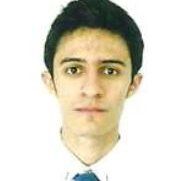
\includegraphics[width = 1.8cm, height = 3.5cm]{img/jeanarreola}
  \section{Dirección}
    Coacalco
    Estado de México
    ~
  \section{Tel}
    +55 37874911
    ~
  \section{Mail}
    \href{mailto:jean.arreola@yahoo.com}{\textbf{jean.arreola@}\\yahoo.com.mx}
    ~
  \section{Github \& Linkedin}
    \href{https://github.com/jean9208}{github.com/jean9208}
    \href{https://www.linkedin.com/in/jean-arreola-trapala/}{linkedin.com/in/jean-arreola-trapala}
    ~
  % use  \hspace{} or \vspace{} to change bubble size, if needed
  \section{Programming}
    \smartdiagram[bubble diagram]{
        \textbf{R},
        \textbf{Python},
        \textbf{C/C++},
        \textbf{SQL},
        \textbf{Neo4j},
        \textbf{Selenium}
    }
    ~
  \section{Skills}
    \smartdiagram[bubble diagram]{
        \textbf{Estadística},
        \textbf{Machine} \\\textbf{Learning},
        \textbf{Web} \\\textbf{Scraping},
        \textbf{Shiny}
    }
    ~
\end{aside}
~
\section{Experiencia}
\begin{entrylist}
  \entry
    {08/17 - actual}
    {Estadístico Freelance}
    {Independiente}
    { \begin{itemize}
         \item Optimización de tarifas para el seguro de auto
      \end{itemize}     }
  \entry
    {11/15 - 07/17}
    {Coordinador Actuarial}
    {HDI Seguros}
    { \begin{itemize}
    
        \item Modelos de renovación de cartera
        \item Shinyapps para mejora de procesos
        \item Implementación de sistema antifraudes con Neo4j
      \end{itemize}       
       }
  \entry
    {07/14 - 10/15}
    {Analista de Tarifas}
    {HDI Seguros}
    { \begin{itemize}
         \item Elaboración de tarifas de seguro de auto con GLM    
         \item Validación actuarial de la información
         \item Forecasting
      \end{itemize}     
     }
    
\end{entrylist}

\section{Educacion}
\begin{entrylist}
  \entry
    {2017 - 2019}
    {Maestría en Cómputo Estadístico}
    {CIMAT Unidad Mty}
    {\begin{itemize}
      \item  Estadística Multivariada
      \item  Aprendizaje de Máquina
      \item  Datos no estructurados
    \end{itemize}}
  \entry
    {2014 - 2015}
    {Diplomado en Finanzas y Técnicas Computacionales}
    {UNAM FES Acatlán}
	{\begin{itemize}
	  \item Portafolios de Inversión
	  \item Derivados financieros
	  \item Riesgos financieros
	\end{itemize} } 
  \entry
    {2010 - 2014}
    {Licenciatura en Actuaría}
    {UNAM FES Acatlán}
    {\begin{itemize}
      \item Probabilidad y Estadística
      \item Programación (R)
      \item Matemáticas Financieras
    \end{itemize}}
\end{entrylist}
\\

\section{Certificaciones}
\begin{entrylist}
  \entry
    {03/2018}
    {Bayesian Methods for Machine Learning}
    {Coursera}
    {\emph{Mezclas Gausianas, Inferencia Variacional y Optimización Bayesiana}}
    
  \entry
    {11/2015}
    {Data Science and Machine Learning Essentials}
    {edX}
    {\emph{Azure ML para aprendizaje supervisado y no supervisado}}
\end{entrylist}

\section{Otra Información}
Colaborador en Rbloggers\\


\end{document}
